

%--------------------------------------------------
Nuestra metodología está organizada por etapas que se alinean con los objetivos específicos del proyecto. El enfoque general consiste en integrar datos, limpiarlos, analizarlos y construir modelos para predecir los indicadores $SAIDI$ y $SAIFI$ de la empresa de distribución eléctrica en Norte de Santander.

Se decidió utilizar CRISP-DM (Cross-Industry Standard Process for Data Mining) como marco de referencia por ser un estándar reconocido en la industria para proyectos de ciencia de datos, el cual fue adaptado al contexto específico del sector eléctrico regulado. Las fases de CRISP-DM se implementaron de la siguiente manera: el entendimiento del negocio (Business Understanding) se desarrolla en las Secciones 1–4, donde se describen el problema, los objetivos y la justificación. Las fases de entendimiento y preparación de datos (Data Understanding y Data Preparation) corresponden a las Etapas 1, 2, 3 y 4, en las que se integran, depuran, exploran los datos y se construyen las variables analíticas. La fase de modelado y evaluación (Modeling y Evaluation) se desarrolla en la Etapa 5, donde se construyen y validan los modelos predictivos. Finalmente, el despliegue (Deployment) corresponde a la Etapa 6, en la cual se consolidan los resultados, se documenta el proceso y se entrega código reproducible.

Esta adaptación de CRISP-DM considera los requisitos específicos del regulador (CREG, SSPD), las métricas propias del sector eléctrico ($SAIDI$, $SAIFI$) y la necesidad de que los modelos sean interpretables para su uso en la toma de decisiones.

\section{Etapa 1 – Extracción de datos}


\textbf{Objetivo específico asociado: OE1}

Esta etapa comprende la recolección, integración y estandarización de las fuentes de datos internas (SCADA, OMS, GIS, CIS, registros de fallas y mantenimiento) y externas (NASA, CREG, SSPD). Incluye la creación de un repositorio analítico unificado y la elaboración de un catálogo de datos que documenta metadatos, alcances, limitaciones y métricas de integridad.

\textbf{Entregable:} Informe de consolidación de datos y catálogo de calidad e integridad.

\subsubsection{Fuentes de informacion}

A partir del año $2023$, la Electrificadora de Norte de Santander realizó una migración de su sistema de gestión de interrupciones. Como resultado, la recopilación de información de interrupciones eléctricas se llevó a cabo a partir de dos bases de datos provenientes de sistemas distintos:

\begin{itemize}
\item \textbf{OMS Energy}: sistema utilizado hasta antes de la migración, del cual se extrae la información histórica de interrupciones previas a $2023$.
\item \textbf{OMS SP7 de Siemens}: nuevo sistema implementado desde $2023$, del cual se obtiene la información de interrupciones a partir de dicha fecha.
\end{itemize}

Esta dualidad de fuentes implica diferencias estructurales en los esquemas de datos (tales como nombres de campos, codificaciones y niveles de granularidad), las cuales fueron consideradas durante el proceso de integración y homologación de la información.


\subsection{Sistemas y fuentes consultadas}

Se integran datos de cinco fuentes de información principales:

\begin{itemize}
\item BRAE: base regulatoria e histórica de eventos.
\item OMS SPARD (sistema histórico): fuente de elemento causante antes de la migración.
\item OMS SP7 (sistema actual): fuente de elemento causante en archivos CSV mensuales.
\item GTECH (GIS): inventario y georreferenciación de activos eléctricos.
\item NASA POWER (API): serie diaria de variables climatológicas por coordenada/cuadrante.
\end{itemize}

\subsection{Extracción base y depuración de eventos de interrupción (BRAE)}

La construcción de la base de eventos de interrupción se realizó a partir de la tabla transaccional \texttt{BRAE.QA\_TFDDREGISTRO}, la cual contiene el registro histórico de eventos de desconexión del sistema eléctrico. A partir de esta fuente, se ejecutó una consulta SQL orientada a depurar inconsistencias, restringir el periodo de análisis y estandarizar la estructura del identificador de evento.

En primer lugar, se seleccionaron únicamente los campos relevantes para el análisis: el identificador del evento (\texttt{FDD\_CODIGOEVENTO}), la fecha de inicio de la desconexión (\texttt{FDD\_FINICIAL}) y la fecha de reconexión (\texttt{FDD\_FFINAL}). Adicionalmente, se incluyó un campo vacío para \texttt{ELEMENTO\_FALLADO}, con el fin de mantener compatibilidad estructural con otras fuentes que sí contienen este nivel de desagregación.

Posteriormente, se aplicaron criterios de depuración y filtrado. En primer lugar, se restringió la muestra al periodo comprendido entre los años 2021 y 2025, garantizando consistencia temporal del análisis. En segundo lugar, se excluyeron aquellos registros marcados como no relevantes mediante la variable \texttt{FDD\_EXCLUSION}, conservando únicamente los eventos clasificados como \texttt{NO EXCLUIDA}. En tercer lugar, se eliminaron eventos asociados a causas no válidas según la regulación (\texttt{FDD\_CAUSA\_SSPD NOT IN (1)}), así como aquellos registros sin fecha de finalización (\texttt{FDD\_FFINAL IS NOT NULL}), los cuales no permiten calcular la duración del evento.

Finalmente, se utilizó la instrucción \texttt{DISTINCT} para garantizar la eliminación de duplicados en el identificador de evento, obteniéndose una base depurada y consistente a nivel de evento de interrupción. Como resultado de este proceso de extracción y limpieza, se obtuvo un total de 95{,}280 registros válidos de eventos de desconexión para el periodo de análisis.

\begin{lstlisting}[style=thesiscode,language=SQL]
SELECT DISTINCT FDD_CODIGOEVENTO AS ID_EVENTO
      ,FDD_FINICIAL AS FECHA_DESCONEXION
      ,FDD_FFINAL AS FECHA_CONEXION
      ,'' AS ELEMENTO_FALLADO
FROM BRAE.QA_TFDDREGISTRO
WHERE TO_CHAR(FDD_FINICIAL,'YYYY') IN ('2021', '2022', '2023', '2024', '2025')
  AND FDD_EXCLUSION = 'NO EXCLUIDA'
  AND FDD_CAUSA_SSPD NOT IN (1)
  AND FDD_FFINAL IS NOT NULL;
\end{lstlisting}

\begin{table}[H]
\centering
\small
\caption{Muestra de eventos depurados de interrupción (BRAE)}
\label{tab:muestra_eventos_brae}
\begin{tabularx}{\textwidth}{>{\raggedright\arraybackslash}p{1.8cm} >{\raggedright\arraybackslash}p{3.7cm} >{\raggedright\arraybackslash}p{3.7cm} >{\raggedright\arraybackslash}p{2.6cm}}
\toprule
\textbf{ID EVENTO} & \textbf{FECHA DESCONEXION} & \textbf{FECHA CONEXION} & \textbf{ELEMENTO FALLADO} \\
\midrule
801851 & 14/03/21 06:59:00.000 & 14/03/21 09:30:00.000 & (null) \\
787583 & 04/01/21 08:50:00.000 & 04/01/21 17:15:00.000 & (null) \\
787496 & 03/01/21 14:18:14.296 & 03/01/21 14:40:42.699 & (null) \\
787232 & 01/01/21 10:29:33.936 & 01/01/21 13:30:00.000 & (null) \\
787455 & 03/01/21 10:34:23.000 & 03/01/21 13:30:00.000 & (null) \\
787376 & 02/01/21 12:09:22.000 & 02/01/21 18:20:00.000 & (null) \\
789756 & 16/01/21 08:50:00.000 & 16/01/21 15:50:00.000 & (null) \\
788677 & 10/01/21 08:37:45.000 & 10/01/21 10:10:00.000 & (null) \\
788932 & 12/01/21 06:47:47.000 & 12/01/21 08:30:00.000 & (null) \\
787922 & 06/01/21 08:42:00.000 & 06/01/21 15:28:00.000 & (null) \\
\bottomrule
\end{tabularx}
\end{table}


\subsection{Extracción de afectación por evento}

Con el fin de complementar la base de eventos de interrupción, se construyó una tabla de afectación asociada a cada evento, incorporando información sobre el número de elementos afectados y la cantidad de usuarios impactados. Este proceso permite pasar de una caracterización puramente temporal del evento a una medición de su severidad en términos de impacto en la red.

La extracción se realizó a partir de la tabla \texttt{BRAE.QA\_TFDDREGISTRO}, la cual se utilizó como fuente principal de eventos, y se complementó mediante una unión (LEFT JOIN) con la base \texttt{QA\_TTC1}, que contiene información asociada a la conexión de transformadores y el número de usuarios por conexión.

En particular, la variable \texttt{CANTIDAD\_USUARIOS} se construyó a partir del conteo de usuarios asociados a cada transformador (\texttt{TC1\_CODCONEX}) agrupados por periodo, mientras que la variable de afectación por evento se obtuvo mediante la agregación de estos usuarios a nivel de evento de interrupción.

Posteriormente, se aplicaron los mismos criterios de depuración utilizados en la etapa anterior, restringiendo el análisis al periodo 2021–2025, excluyendo eventos marcados como no relevantes (\texttt{FDD\_EXCLUSION = 'NO EXCLUIDA'}), eliminando causas no válidas según la clasificación regulatoria (\texttt{FDD\_CAUSA\_SSPD NOT IN (1)}) y conservando únicamente registros con fecha de finalización válida (\texttt{FDD\_FFINAL IS NOT NULL}).

Finalmente, los datos se agregaron a nivel de evento (\texttt{FDD\_CODIGOEVENTO}) utilizando la función \texttt{GROUP BY}, obteniendo como resultado dos indicadores clave: el número de elementos fallados por evento y el total de usuarios afectados. El procedimiento permitió consolidar una base consistente de 95{,}280 registros, alineada con la estructura del conjunto de eventos previamente depurado.

\begin{lstlisting}[style=thesiscode,language=SQL]
SELECT FDD_CODIGOEVENTO AS ID_EVENTO
      ,COUNT(FDD_CODIGOELEMENTO) AS CANTIDAD_ELEMENTOS_FALLADOS
      ,SUM(CANTIDAD_USUARIOS) AS CANTIDAD_USUARIOS
FROM BRAE.QA_TFDDREGISTRO
LEFT JOIN (
    SELECT TC1_CODCONEX AS TRANSFORMADOR
          ,COUNT(TC1_CODCONEX) AS CANTIDAD_USUARIOS
          ,TC1_PERIODO AS PERIODO
    FROM QA_TTC1
    WHERE SUBSTR(TC1_PERIODO, 1, 4) IN ('2021', '2022', '2023', '2024', '2025')
    GROUP BY TC1_PERIODO, TC1_CODCONEX
) ON FDD_CODIGOELEMENTO = TRANSFORMADOR
 AND FDD_PERIODO_TC1 = PERIODO
WHERE TO_CHAR(FDD_FINICIAL,'YYYY') IN ('2021', '2022', '2023', '2024', '2025')
  AND FDD_EXCLUSION = 'NO EXCLUIDA'
  AND FDD_CAUSA_SSPD NOT IN (1)
  AND FDD_FFINAL IS NOT NULL
GROUP BY FDD_CODIGOEVENTO;
\end{lstlisting}

\begin{table}[H]
\centering
\small
\caption{Muestra de afectación por evento (BRAE + QA\_TTC1)}
\label{tab:muestra_afectacion_evento}
\begin{tabularx}{0.9\textwidth}{
    >{\raggedright\arraybackslash}p{2.0cm}
    >{\centering\arraybackslash}p{4.6cm}
    >{\centering\arraybackslash}p{3.0cm}
}
\toprule
\textbf{ID EVENTO} & \textbf{CANTIDAD ELEMENTOS FALLADOS} & \textbf{CANTIDAD USUARIOS AFECTADOS} \\
\midrule
795044 & 33  & 2692  \\
795513 & 162 & 11796 \\
788221 & 10  & 74    \\
788203 & 240 & 3865  \\
789543 & 8   & 45    \\
789719 & 109 & 503   \\
789929 & 109 & 503   \\
788758 & 1   & 6     \\
798712 & 159 & 1869  \\
\bottomrule
\end{tabularx}
\end{table}

\subsection{Extracción del elemento causante histórico}

Con el objetivo de identificar el elemento de la red asociado a la causa de cada evento de maniobra, se realizó la extracción de información histórica desde la base de datos del sistema OMS (Outage Management System), específicamente desde la tabla \texttt{OMS.MANIOBRAS@SPARD}. Esta fuente permite complementar la información de eventos de interrupción mediante la identificación del elemento físico que originó la falla.

El proceso de extracción se centró en dos variables principales: el código de la maniobra (\texttt{CODE}), utilizado como identificador del evento en el sistema OMS, y el elemento fallado (\texttt{BREAKER}), que corresponde al activo de la red asociado a la causa de la interrupción. Estas variables permiten establecer la relación entre el evento registrado y el componente físico responsable dentro de la infraestructura eléctrica.

Adicionalmente, se aplicaron criterios de filtrado temporal y de calidad de datos. En primer lugar, se restringió la información a registros con fecha igual o posterior al año 2021, garantizando la consistencia histórica del análisis. En segundo lugar, se excluyeron aquellos eventos clasificados como pruebas operativas mediante la condición \texttt{CAUSA != 'PRUEBA'}, con el fin de conservar únicamente eventos reales de operación del sistema.

Como resultado de este proceso de extracción y depuración, se obtuvo una base de datos estructurada a nivel de maniobra, la cual permite complementar la trazabilidad entre eventos de interrupción y los elementos físicos de la red asociados a su ocurrencia.

\begin{lstlisting}[style=thesiscode,language=SQL]
SELECT CODE AS CODIGO_MANIOBRA
      ,BREAKER AS ELEMENTO_FALLADO
FROM OMS.MANIOBRAS@SPARD
WHERE TO_NUMBER(TO_CHAR(FECHA, 'YYYY')) >= 2021
  AND CAUSA != 'PRUEBA';
\end{lstlisting}

\begin{table}[H]
\centering
\small
\caption{Muestra de elemento causante histórico (OMS SPARD)}
\label{tab:muestra_elemento_causante_historico}
\begin{tabularx}{0.72\textwidth}{>{\centering\arraybackslash}p{3.0cm} >{\centering\arraybackslash}p{4.0cm}}
\toprule
\textbf{CODIGO MANIOBRA} & \textbf{ELEMENTO FALLADO} \\
\midrule
640011 & AMVE271 \\
634924 & LMVEL79620 \\
634978 & LMVEL67393 \\
631108 & RMVEL79067-2 \\
631464 & CMVE2454 \\
631761 & SW6844 \\
637873 & BMVE749 \\
640442 & LMVEL99259 \\
631793 & SANC52 \\
\bottomrule
\end{tabularx}
\end{table}

\subsection{Extracción del elemento causante actual}

Con el objetivo de actualizar la información histórica del sistema de maniobras, se realizó la extracción de los datos correspondientes a la versión más reciente del sistema OMS en formato plano (CSV). Este proceso permite complementar la información histórica con registros operativos actuales, garantizando la continuidad y consistencia de la base de datos utilizada en el análisis.

La extracción se realizó mediante un proceso de lectura y depuración de datos en Python, a partir del archivo fuente correspondiente a la versión actual del sistema. En primer lugar, se cargó el archivo mediante la función \texttt{read\_csv}, asegurando la correcta lectura de la estructura tabular. Posteriormente, se realizó una limpieza de los nombres de las columnas mediante la eliminación de espacios en blanco al inicio y al final, con el fin de evitar inconsistencias en la identificación de variables.

A continuación, se seleccionaron únicamente las variables relevantes para el análisis: \texttt{Maniobra Apertura}, \texttt{Tipo Elemento} y \texttt{Elemento\_Falla}. Esta selección permitió homogenizar la estructura de la base con la información histórica previamente construida. Finalmente, se eliminaron los registros duplicados mediante la función \texttt{drop\_duplicates}, garantizando la unicidad de las observaciones a nivel de combinación de variables relevantes.

Como resultado, se obtuvo una base depurada y estandarizada del sistema OMS actual, la cual es consistente con la estructura de la base histórica y permite su integración en el proceso de consolidación del dataset final.

\begin{lstlisting}[style=thesiscode,language=Python]
columnas_necesarias = ['Maniobra Apertura', 'Tipo Elemento', 'Elemento_Falla']
df = pd.read_csv(ruta_actual)
df.columns = df.columns.str.strip()
df = df[columnas_necesarias].drop_duplicates()
\end{lstlisting}

\begin{table}[H]
\centering
\small
\caption{Muestra de elemento causante actual (OMS SP7)}
\label{tab:muestra_elemento_causante_actual}
\begin{tabularx}{0.95\textwidth}{
    >{\centering\arraybackslash}p{3.8cm} 
    >{\raggedright\arraybackslash}p{4.8cm} 
    >{\centering\arraybackslash}p{2.7cm}}
\toprule
\textbf{MANIOBRA APERTURA} & \textbf{TIPO ELEMENTO} & \textbf{ELEMENTO FALLA} \\
\midrule
424000000000114424 & Transformador de distribucion & 1T07942 \\
124000000000269842 & Fusible & F1979 \\
124000000000269842 & Transformador de distribucion & F1979 \\
124000000000273378 & Fusible & F2004 \\
124000000000269851 & Fusible & F2000 \\
124000000000273383 & Fusible & F2001 \\
124000000000273374 & Fusible & F2006 \\
124000000000273377 & Fusible & F2004 \\
124000000000273372 & Fusible & F2006 \\
124000000000273356 & Fusible & F2005 \\
124000000000273381 & Fusible & F1993 \\
\bottomrule
\end{tabularx}
\end{table}

\subsection{Extracción de inventario GIS}

Con el propósito de incorporar la dimensión espacial de la red eléctrica, se realizó la extracción del inventario georreferenciado a partir del sistema GIS corporativo. Esta información permite asociar cada activo de la red con sus coordenadas geográficas y características físicas, facilitando posteriormente el análisis espacial de los eventos de interrupción.

La extracción se efectuó desde la base de datos \texttt{ccomun@gtech}, la cual contiene el inventario técnico de los activos de la red. A partir de esta fuente, se seleccionaron las variables correspondientes al identificador del elemento (\texttt{nodo\_transform\_v}), la latitud (\texttt{coor\_gps\_lat}), la longitud (\texttt{coor\_gps\_lon}) y la altitud (\texttt{coor\_z}). Adicionalmente, se incluyó la variable \texttt{ubicacion}, que permite complementar la caracterización espacial del activo.

Asimismo, se definió explícitamente el tipo de activo como \texttt{Transformador}, con el fin de estandarizar la clasificación dentro del conjunto de datos integrado. Esta homogenización resulta clave para la posterior vinculación con los eventos de interrupción y la construcción del panel activo–día.

Como resultado, se obtuvo una base georreferenciada de los activos de la red, la cual constituye un insumo fundamental para el enriquecimiento espacial del dataset consolidado.

\begin{lstlisting}[style=thesiscode,language=SQL]
SELECT 
    nodo_transform_v AS ELEMENTO,
    coor_gps_lat     AS LATITUD,
    coor_gps_lon     AS LONGITUD,
    coor_z           AS ALTITUD,
    'Transformador'  AS TIPO,
    ubicacion
FROM ccomun@gtech c
JOIN cconectividad_e@gtech USING (g3e_fid)
WHERE c.estado = 'OPERACION'
  AND c.g3e_fno = 20400
UNION
SELECT 
    r.codigo         AS ELEMENTO,
    coor_gps_lat     AS LATITUD,
    coor_gps_lon     AS LONGITUD,
    coor_z           AS ALTITUD,
    'Reconectador'   AS TIPO,
    ubicacion
FROM ereconec_at@gtech r
JOIN ccomun@gtech c USING (g3e_fid)
JOIN cconectividad_e@gtech USING (g3e_fid)
WHERE c.estado = 'OPERACION';

\end{lstlisting}

\begin{table}[H]
\centering
\footnotesize
\setlength{\tabcolsep}{3pt}
\renewcommand{\arraystretch}{1.05}
\caption{Muestra de inventario georreferenciado de activos (GIS GTECH)}
\label{tab:muestra_inventario_gis}
\begin{tabularx}{\textwidth}{
>{\raggedright\arraybackslash}p{1.5cm}
>{\centering\arraybackslash}p{2.2cm}
>{\centering\arraybackslash}p{2.2cm}
>{\centering\arraybackslash}p{1.2cm}
>{\centering\arraybackslash}X
}
\toprule
\textbf{ELEMENTO} & \textbf{LATITUD} & \textbf{LONGITUD} & \textbf{ALTITUD} & \textbf{TIPO} \\
\midrule
2T01558 & 6.960719612 & -72.18029066 & 636 & Transformador \\
2T01557 & 6.972762106 & -72.18726993 & 743 & Transformador \\
2T01467 & 6.973200989 & -72.15472768 & 815 & Transformador \\
2T01466 & 6.978510343 & -72.14903608 & 726 & Transformador \\
F3199   & 6.978980206 & -72.19049387 & 832 & Aisladero \\
PSW8910 & 6.978980206 & -72.19049387 & 832 & Aisladero \\
2T01555 & 6.982222682 & -72.19495813 & 825 & Transformador \\
2T01554 & 6.982742594 & -72.20226264 & 867 & Transformador \\
2T01556 & 6.984663810 & -72.18619273 & 727 & Transformador \\
2T01465 & 6.985402944 & -72.13537905 & 530 & Transformador \\
F3192   & 6.987527091 & -72.20044897 & 767 & Aisladero \\
PSW8909 & 6.987527091 & -72.20044897 & 767 & Aisladero \\
F5217   & 6.991040416 & -72.20123180 & 726 & Aisladero \\
PSW8908 & 6.991040416 & -72.20123180 & 726 & Aisladero \\
2T01553 & 6.991242376 & -72.19636467 & 679 & Transformador \\
2T01470 & 6.991396285 & -72.15644527 & 790 & Transformador \\
ESW6924 & 6.992103744 & -72.13486380 & 453 & Aisladero \\
F5211   & 6.992103744 & -72.13486380 & 453 & Aisladero \\
2T01471 & 6.992290614 & -72.13485446 & 453 & Transformador \\
2T01469 & 6.993224220 & -72.14776723 & 656 & Transformador \\
F8201   & 6.997255476 & -72.12409341 & 361 & Aisladero \\
\bottomrule
\end{tabularx}
\end{table}

Y asi sucesivamente para Interruptor, Cuchilla, Aisladero, Reconectador y Transformador.

\subsection{Extracción de variables meteorológicas}

Con el objetivo de incorporar condiciones climáticas como variables explicativas en el análisis de interrupciones del sistema eléctrico, se realizó la extracción de información meteorológica a partir de la plataforma NASA POWER. Esta fuente proporciona series temporales diarias de variables climáticas relevantes, las cuales permiten capturar la influencia del entorno atmosférico sobre la ocurrencia y duración de eventos en la red.

El proceso de extracción se centró en un conjunto de variables meteorológicas seleccionadas por su relevancia en el análisis de confiabilidad del sistema eléctrico. En particular, se consideraron las variables de precipitación total (\texttt{PRECTOT}), temperatura media (\texttt{T2M}), temperatura máxima (\texttt{T2M\_MAX}), temperatura mínima (\texttt{T2M\_MIN}), humedad relativa (\texttt{RH2M}) y velocidad del viento (\texttt{WS2M}).

\begin{lstlisting}[style=code,language=Python]
parametros_nasa = ("PRECTOT", "T2M", "T2M_MAX", "T2M_MIN", "RH2M", "WS2M")
\end{lstlisting}

\begin{table}[H]
\centering
\small
\caption{Muestra de variables meteorológicas (NASA POWER) - Parte 1}
\label{tab:muestra_nasa_power_1}
\begin{tabularx}{\textwidth}{
>{\centering\arraybackslash}p{2.0cm}
>{\centering\arraybackslash}p{2.0cm}
>{\centering\arraybackslash}p{2.0cm}
>{\centering\arraybackslash}p{2.0cm}
>{\centering\arraybackslash}p{2.0cm}
>{\centering\arraybackslash}p{2.0cm}
}
\toprule
\textbf{VEL. VIENTO} & \textbf{TEMP. MEDIA} & \textbf{HUMEDAD} & \textbf{TEMP. MIN} & \textbf{TEMP. MAX} & \textbf{PRECIP.} \\
\midrule
2.06 & 13.27 & 87.24 & 9.12 & 18.63 & 2.6  \\
2.66 & 13.89 & 88.27 & 10.71 & 18.92 & 1.41 \\
1.93 & 13.66 & 88.59 & 10.29 & 18.96 & 3.04 \\
1.73 & 13.6  & 85.07 & 9.13 & 20.17 & 9.07 \\
1.45 & 11.52 & 69.12 & 5.95 & 18.7  & 0.79 \\
1.1  & 12.29 & 80.8  & 7.55 & 17.76 & 0.77 \\
1.76 & 13.23 & 88.9  & 10.65 & 17.93 & 3.03 \\
2.34 & 12.95 & 88.44 & 10.14 & 17.84 & 2.51 \\
2.41 & 12.69 & 87.38 & 9.48 & 16.55 & 1.84 \\
2.98 & 12.99 & 90.13 & 9.65 & 17.44 & 3.35 \\
3.18 & 13.12 & 87.67 & 10.58 & 17.69 & 0.9  \\
\bottomrule
\end{tabularx}
\end{table}

Estas variables fueron extraídas a nivel diario para el periodo comprendido entre el 1 de enero de 2021 y el 31 de diciembre de 2025, lo que dio lugar a una base de aproximadamente 83.5 millones de registros. Este volumen de información refleja la estructura panelizada de la base climática, construida mediante la combinación de múltiples variables atmosféricas observadas diariamente a lo largo del horizonte temporal de análisis.

La incorporación de estas variables permite enriquecer el dataset consolidado con condiciones exógenas del entorno, facilitando el análisis de su relación con la frecuencia y severidad de las interrupciones en el sistema eléctrico.

\subsection{Resumen metodológico de extracción e integración de bases de datos}

\begin{table}[ht]
\centering
\small
\caption{Resumen metodológico de extracción e integración de bases de datos}
\label{tab:data_lineage}
\begin{tabular}{p{3.5cm} p{3cm} p{3cm} p{3cm}}
\hline
\textbf{Fuente} & \textbf{Variables principales} & \textbf{Proceso aplicado} & \textbf{Resultado} \\
\hline

BRAE (QA\_TFDDREGISTRO) 
& ID EVENTO, FECHA DESCONEXION, FECHA CONEXION 
& Filtrado temporal (2021–2025), exclusión de registros no válidos, eliminación de duplicados 
& 95.280 eventos de interrupción \\

\hline

BRAE + QA\_TTC1 
& CANTIDAD USUARIOS, ELEMENTOS DE CONEXION 
& JOIN por elemento y periodo, agregación por evento 
& Base de severidad por evento (usuarios) \\

\hline

OMS SPARD (histórico) 
& CODIGO MANIOBRA, ELEMENTO FALLADO, ELEMENTO CAUSANTE 
& Filtrado de registros desde 2021, exclusión de pruebas 
& Base histórica de causa de falla \\

\hline

OMS SP7 (actual) 
& MANIOBRA APERTURA, TIPO ELEMENTO, CANTIDAD ELEMENTOS FALLADOS, ELEMENTO FALLA 
& Lectura CSV, limpieza de columnas, eliminación de duplicados 
& Base actualizada de elementos causantes \\

\hline

GIS (GTECH) 
& ELEMENTO, LATITUD, LONGITUD, ALTITUD, TIPO 
& Extracción desde sistema georreferenciado corporativo 
& Inventario espacial de la red \\

\hline

NASA POWER 
& PRECTOT, T2M, T2M\_MAX, T2M\_MIN, RH2M, WS2M 
& Extracción diaria (2021–2025) por variables climáticas 
& 83.5 millones de registros meteorológicos \\

\hline
\end{tabular}
\end{table}
Lógica de in
La Tabla~\ref{tab:data_lineage} sintetiza el proceso de extracción e integración desarrollado en la Etapa~1. En conjunto, se consolidaron seis fuentes complementarias: BRAE como base transaccional de eventos de interrupción; BRAE + QA\_TTC1 para cuantificar la severidad operativa (usuarios afectados); OMS SPARD y OMS SP7 para identificar el elemento causante y fallado en los periodos pre y post migración del sistema; GIS (GTECH) para incorporar la georreferenciación de activos de red; y NASA POWER para enriquecer el análisis con variables climáticas diarias. Cada fuente fue sometida a reglas explícitas de filtrado, homologación y depuración, lo que permitió obtener bases consistentes y trazables que constituyen el insumo inicial para la integración y el preprocesamiento descritos en la Etapa~2.




\section{Etapa 2 - Integración, depuración y preprocesamiento de datos}

\subsection{Lógica de integración entre sistemas}

Una vez extraídas y depuradas las fuentes descritas en la Etapa~1, la integración se ejecuta de forma secuencial sobre tablas intermedias, preservando trazabilidad de llaves y evitando pérdida de emparejamiento entre sistemas con esquemas distintos (BRAE, OMS SPARD, OMS SP7, GIS y NASA POWER). La secuencia aplicada fue la siguiente:

{\sloppy
\renewcommand{\theenumi}{\thesubsection.\arabic{enumi}}
\renewcommand{\labelenumi}{\theenumi}
\begin{enumerate}
    \item \label{int:paso1} \textbf{Construcción de la tabla base de eventos (BRAE).}\mbox{}\par\vspace{0.2em}\noindent
    A partir de \texttt{BRAE.QA\_TFDDREGISTRO} se genera la tabla \texttt{tabla\_eventos} con \texttt{ID\_EVENTO}, \texttt{FECHA\_DESCONEXION} y \texttt{FECHA\_CONEXION}, aplicando filtros regulatorios del periodo 2021--2025, exclusión de eventos no válidos y eliminación de duplicados. Esta tabla define el universo analítico de interrupciones (95{,}280 eventos).

    \item \label{int:paso2} \textbf{Construcción de la tabla de afectación por evento (Tabla~5.2).}\mbox{}\par\vspace{0.2em}\noindent
    En la Sección~5.1.3 se construye la Tabla~5.2 de afectación por evento, la cual consolida las columnas \texttt{CANTIDAD\_ELEMENTOS} y \texttt{CANTIDAD\_USUARIOS} a nivel de \texttt{ID\_EVENTO}. Su integración a la tabla base consolidada se realiza en el paso~\ref{int:paso5}.

    \item \label{int:paso3} \textbf{Completar \texttt{ELEMENTO\_FALLADO} (OMS SPARD + OMS SP7).}\mbox{}\par\vspace{0.2em}\noindent
    La tabla base de eventos obtenida en la Sección~5.1.2 se construyó con el campo \texttt{ELEMENTO\_FALLADO} vacío, reservado para su completamiento en la integración. Dado el cambio de sistema OMS en el año 2023, la información del elemento causante se extrajo de forma separada en dos fuentes: la Sección~5.1.4 (\emph{Extracción del elemento causante histórico}, OMS SPARD) y la Sección~5.1.5 (\emph{Extracción del elemento causante actual}, OMS SP7). En este paso, la tabla de la Sección~5.1.2 se cruza con ambas tablas OMS, aplicando en cada caso la lógica de emparejamiento definida en su extracción:
    \begin{itemize}
        \item \emph{Histórico (Sección~5.1.4 -- OMS SPARD):} cruce por \texttt{CODIGO\_MANIOBRA} $\leftrightarrow$ \texttt{ID\_EVENTO} para completar \texttt{ELEMENTO\_FALLADO} con el valor de \texttt{BREAKER} en eventos del periodo pre-migración.
        \item \emph{Actual (Sección~5.1.5 -- OMS SP7):} cruce por \texttt{MANIOBRA\_APERTURA} $\leftrightarrow$ \texttt{ID\_EVENTO} para completar \texttt{ELEMENTO\_FALLADO} con el valor de \texttt{ELEMENTO\_FALLA}, junto con \texttt{TIPO\_ELEMENTO}, en eventos del periodo post-migración.
    \end{itemize}

    \item \label{int:paso4} \textbf{Construcción de la tabla base consolidada (activo--día).}\mbox{}\par\vspace{0.2em}\noindent
    A partir de este paso se inicia la construcción de la tabla base consolidada del proyecto. Como insumo inicial se toma la Tabla~5.5 (inventario georreferenciado de activos obtenido en la Sección~5.1.6), la cual se cruza con un calendario diario comprendido entre el 2021-01-01 y el 2025-12-31, empleando el campo \texttt{FECHA\_DIA}. Este cruce genera un producto cartesiano entre el universo de activos eléctricos y el horizonte temporal de análisis, definiendo la estructura panel \textbf{activo $\times$ día} sobre la cual, en los pasos~\ref{int:paso5} a~\ref{int:paso8}, se anexan los valores restantes de la secuencia de integración.

    \item \label{int:paso5} \textbf{Integración de \texttt{CANTIDAD\_ELEMENTOS} y \texttt{CANTIDAD\_USUARIOS} (Tabla~5.2).}\mbox{}\par\vspace{0.2em}\noindent
    Sobre la tabla base consolidada obtenida en el paso~\ref{int:paso4}, se integran las columnas \texttt{CANTIDAD\_ELEMENTOS} y \texttt{CANTIDAD\_USUARIOS} provenientes de la Tabla~5.2 (afectación por evento, Sección~5.1.3), mediante el siguiente cruce de llaves:
    \begin{itemize}
        \item \texttt{ID\_EVENTO} $=$ \texttt{ELEMENTO}
    \end{itemize}
    \noindent entre la Tabla~5.2 y la tabla del paso~\ref{int:paso4}, incorporando al panel las métricas de severidad e impacto operativo asociadas a cada evento de interrupción.

    \item \label{int:paso6} \textbf{Integración de variables climáticas (NASA POWER).}\mbox{}\par\vspace{0.2em}\noindent
    Sobre la tabla resultante del paso~\ref{int:paso5}, se anexan las variables de la serie diaria \texttt{nasa\_power\_consolidado} mediante cruce por \texttt{FECHA\_DIA}, incorporando precipitación, temperatura (media, máxima, mínima), humedad relativa y velocidad del viento.

    \item \label{int:paso7} \textbf{Agregación de eventos a grano activo--día.}\mbox{}\par\vspace{0.2em}\noindent
    En este paso se construyen las columnas \texttt{DURACION} y \texttt{FRECUENCIA} sobre la tabla resultante del paso~\ref{int:paso6}. Para ello, dicha tabla se cruza con la Tabla~5.1 (eventos depurados de interrupción, Sección~5.1.2), la cual contiene los campos \texttt{FECHA\_DESCONEXION} y \texttt{FECHA\_CONEXION}, mediante la llave:
    \begin{itemize}
        \item \texttt{ID\_EVENTO} $=$ \texttt{ELEMENTO}
    \end{itemize}
    \noindent entre la Tabla~5.1 y el identificador de activo de la tabla del paso~\ref{int:paso6}. Con base en las fechas de desconexión y reconexión, se asignan los valores diarios de la siguiente forma:
    \begin{itemize}
        \item \texttt{DURACION}: para cada activo y \texttt{FECHA\_DIA}, se registra la suma de horas sin servicio efectivamente transcurridas en ese día. Si un evento cruza la medianoche, la duración total se distribuye (prorratea) entre los días calendario en los que el activo permaneció desconectado.
        \item \texttt{FRECUENCIA}: para cada activo y \texttt{FECHA\_DIA}, se registra el número de desconexiones cuyo inicio ocurre en ese día, con base en \texttt{FECHA\_DESCONEXION}. La frecuencia se contabiliza únicamente en el día de ocurrencia del evento, aun cuando la interrupción se extienda a días posteriores; en esos casos, la duración continúa distribuyéndose en los días sucesivos mediante la regla de \texttt{DURACION}.
    \end{itemize}
    \noindent Cuando el activo no presenta interrupciones en un día, se asigna \texttt{DURACION = 0} y \texttt{FRECUENCIA = 0}. 

    \item \label{int:paso8} \textbf{Consolidación del panel final (activo--día).}\mbox{}\par\vspace{0.2em}\noindent
    Sobre la tabla base consolidada definida en el paso~\ref{int:paso4}, y una vez anexados los valores de los pasos~\ref{int:paso5} a~\ref{int:paso7}, se obtiene el dataset final con grano \textbf{activo eléctrico $\times$ día} y $N = 87{,}014{,}378$ observaciones teóricas ($A = 47{,}653$ activos $\times$ $T = 1{,}826$ días). En días sin falla se registra \texttt{DURACION = 0}, \texttt{FRECUENCIA = 0}, \texttt{CANTIDAD\_ELEMENTOS = 0} y \texttt{CANTIDAD\_USUARIOS = 0}.

    La base de datos consolidada se estructura como un panel de datos de tipo activo–tiempo, donde la unidad muestral corresponde a un \textbf{activo eléctrico observado diariamente}. En términos formales, cada observación se identifica mediante el par $(i,t)$, donde $i$ denota el activo eléctrico y $t$ el día dentro del periodo de análisis. Bajo esta estructura, el conjunto de datos permite capturar la evolución temporal de cada activo a lo largo del horizonte de estudio.

Sea $A$ el número total de activos eléctricos en la red y $T$ el número total de periodos diarios observados, el tamaño teórico del panel balanceado está dado por:

\[
N = A \times T
\]

donde:
\begin{itemize}
    \item $A = 47{,}653$ corresponde al número total de activos eléctricos de la red,
    \item $T = 1{,}826$ corresponde al número de días observados (cinco años de información diaria).
\end{itemize}

En consecuencia, el número total de observaciones en la base consolidada se calcula como:

\[
N = 47{,}653 \times 1{,}826 = 87{,}014{,}378
\]


\end{enumerate}
}


\subsection{Diagrama de flujo de la secuencia de integración}

Este diagrama de flujo resume visualmente la secuencia de integración y la estructura del panel final, como guía para el lector, especificando las relaciones entre las tablas y las operaciones aplicadas en cada paso.

\begin{figure}[H]
    \centering
    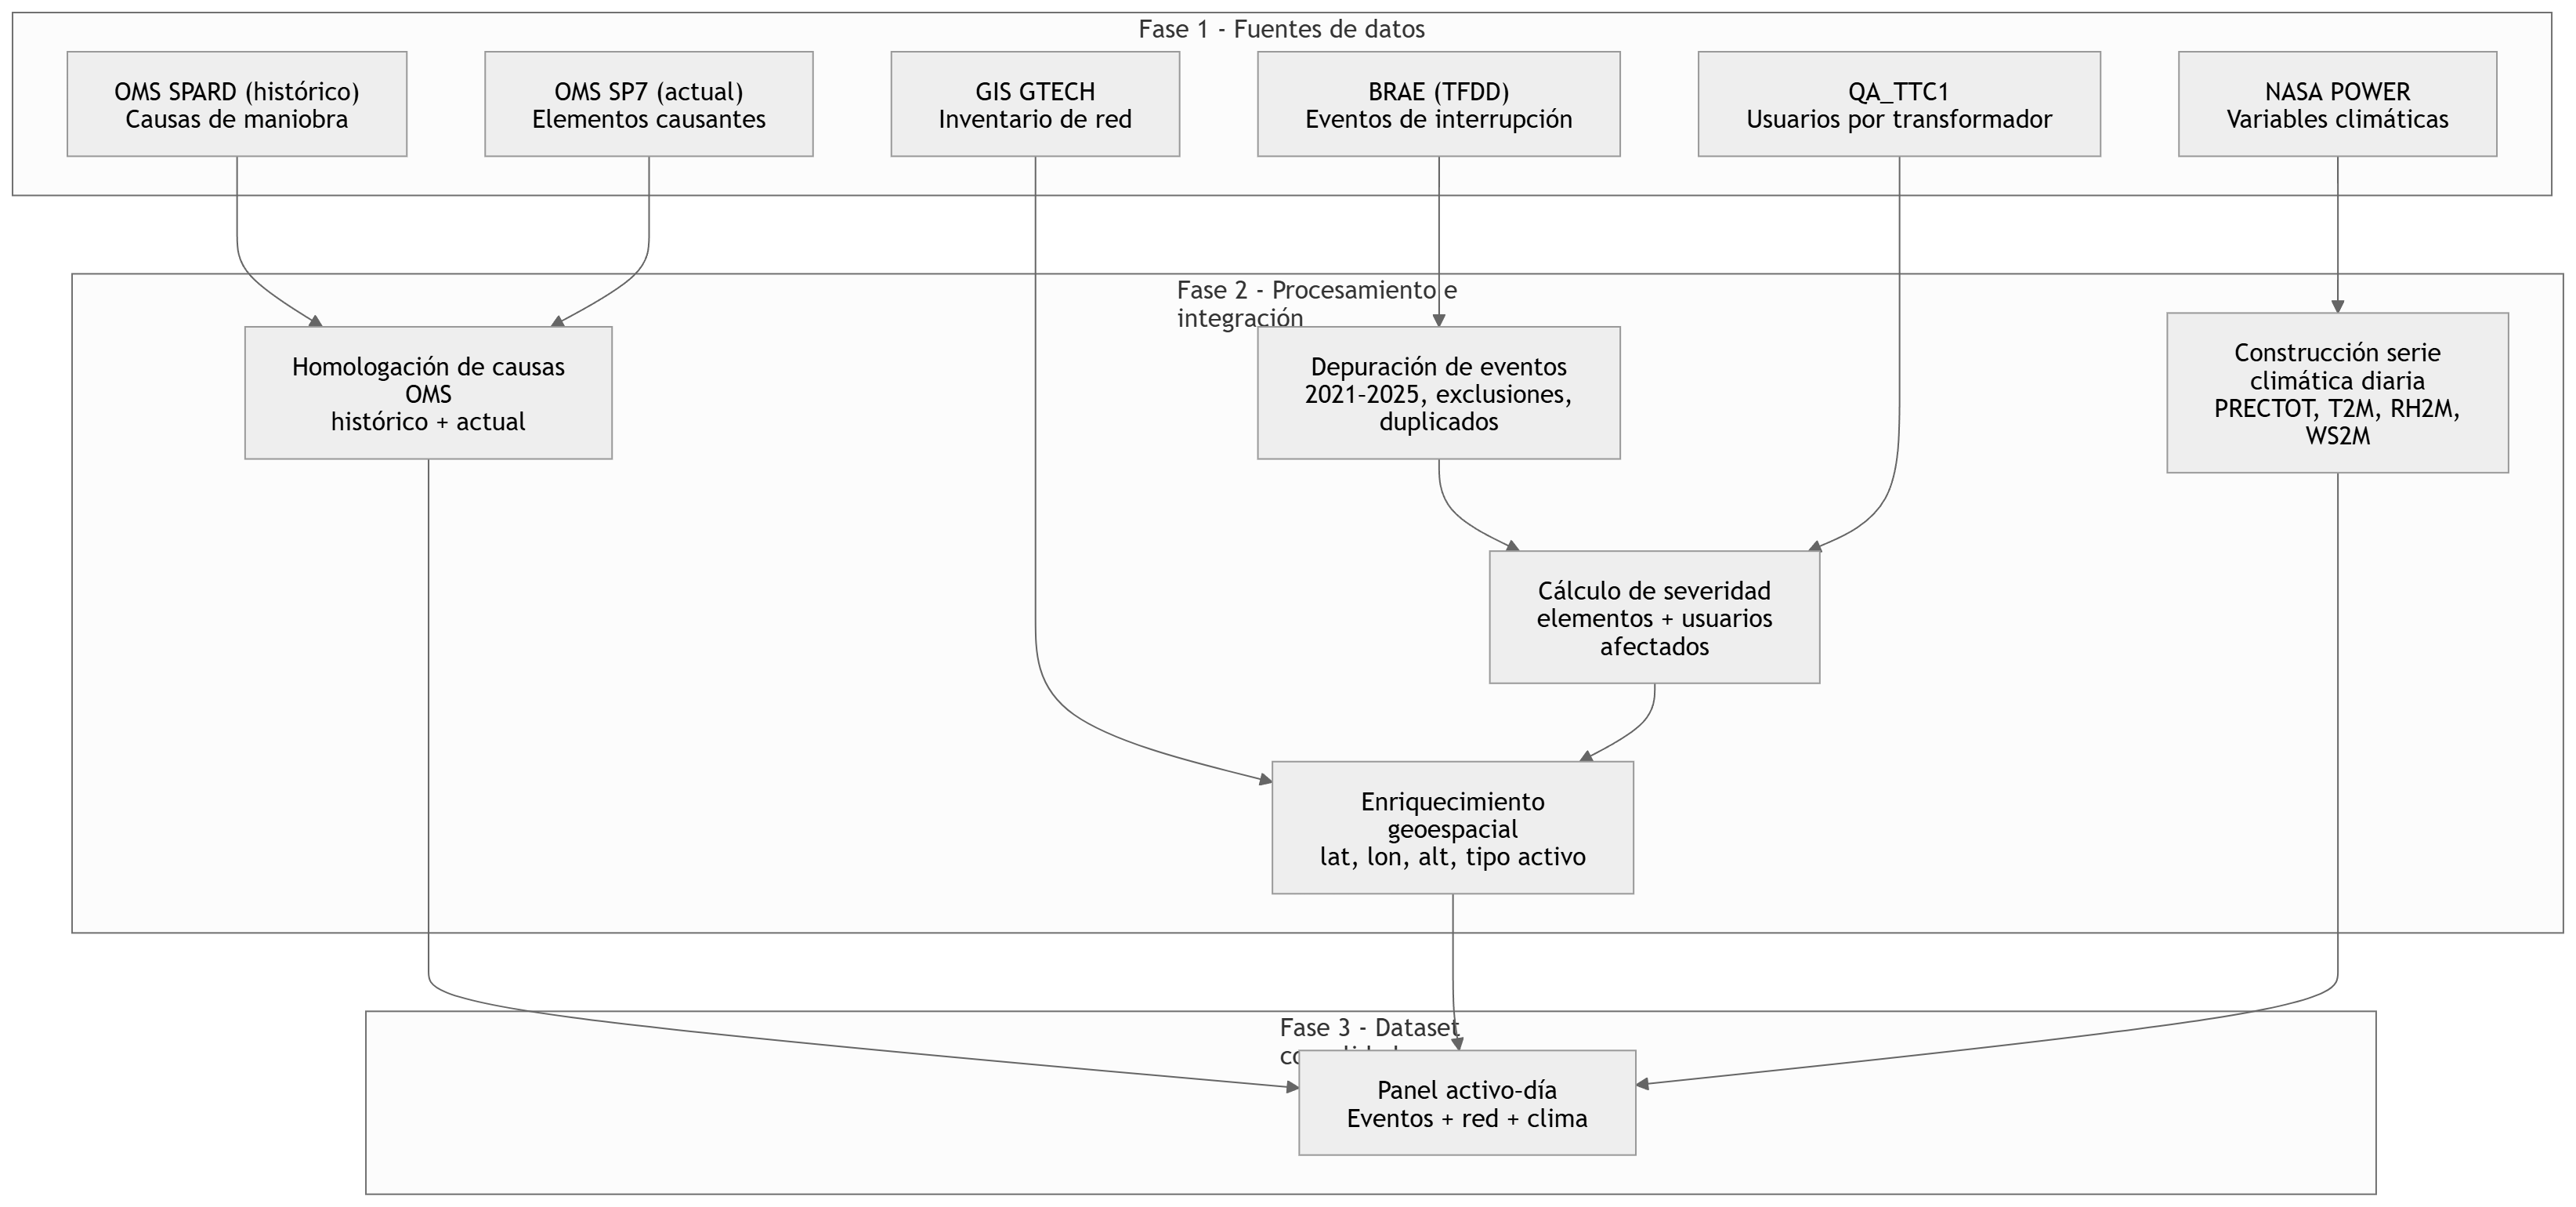
\includegraphics[width=1\textwidth]{img/drawings/mermaid-diagram (1).png}
    \caption{Estructura del panel de datos activo–día}
    \label{fig:panel_activo_dia}
\end{figure}


\subsection{Descripción de la tabla base consolidada}

Las Tablas~\ref{tab:muestra_consolidado_final_1} a~\ref{tab:muestra_consolidado_final_4} presentan una muestra de la tabla base consolidada resultante del paso~\ref{int:paso8}, con grano \textbf{activo eléctrico $\times$ día}. Por limitaciones de ancho en la página, la muestra se divide en cuatro bloques consecutivos que conservan el mismo orden de filas: identificación del activo (Tabla~\ref{tab:muestra_consolidado_final_1}), severidad y clima inicial (Tabla~\ref{tab:muestra_consolidado_final_2}), clima complementario (Tabla~\ref{tab:muestra_consolidado_final_3}) y variables de continuidad (Tabla~\ref{tab:muestra_consolidado_final_4}).

\begin{table}[H]
\centering
\small
\caption{Muestra de la tabla base consolidada (grano activo--día) -- Parte 1: activo y fecha}
\label{tab:muestra_consolidado_final_1}
\begin{tabular}{l l r r r l}
\toprule
\textbf{ID ACTIVO} & \textbf{TIPO} & \textbf{LAT.} & \textbf{LON.} & \textbf{ALT.} & \textbf{FECHA DIA} \\
\midrule
AASW4819 & Aisladero      & 8.5786778 & -72.92349 & 219  & 01/01/2021 \\
1T12452  & Transformador  & 8.5839989 & -72.92248 & 241  & 01/01/2021 \\
REC21365 & Reconectador   & 8.5840628 & -72.92246 & 241  & 01/01/2021 \\
CUC12345 & Cuchilla       & 7.7523729 & -73.23971 & 1236 & 01/01/2021 \\
INT39845 & Interruptor    & 7.7476080 & -73.25551 & 1359 & 02/01/2021 \\
AASW4820 & Aisladero      & 7.7561057 & -73.26037 & 1169 & 02/01/2021 \\
1T12453  & Aisladero      & 7.7409332 & -73.20825 & 1636 & 02/01/2021 \\
REC21366 & Transformador  & 7.7428641 & -73.18990 & 1542 & 02/01/2021 \\
CUC12346 & Reconectador   & 7.7538839 & -73.17721 & 1707 & 03/01/2021 \\
\bottomrule
\end{tabular}
\end{table}

\begin{table}[H]
\centering
\small
\caption{Muestra de la tabla base consolidada (grano activo--día) -- Parte 2: severidad y clima inicial (continuación)}
\label{tab:muestra_consolidado_final_2}
\begin{tabular}{l l r r r r}
\toprule
\textbf{ID ACTIVO} & \textbf{FECHA DIA} & \textbf{C. ELEM.} & \textbf{C. USU.} & \textbf{VEL. VIENTO} & \textbf{TEMP. MED.} \\
\midrule
AASW4819 & 01/01/2021 & 0   & 0    & 1.11 & 23.91 \\
1T12452  & 01/01/2021 & 0   & 0    & 1.23 & 24.58 \\
REC21365 & 01/01/2021 & 125 & 2015 & 0.96 & 23.04 \\
CUC12345 & 01/01/2021 & 0   & 0    & 0.81 & 23.02 \\
INT39845 & 02/01/2021 & 0   & 0    & 1.05 & 23.83 \\
AASW4820 & 02/01/2021 & 0   & 0    & 1.12 & 24.08 \\
1T12453  & 02/01/2021 & 0   & 0    & 1.08 & 24.52 \\
REC21366 & 02/01/2021 & 0   & 0    & 1.26 & 24.37 \\
CUC12346 & 03/01/2021 & 0   & 0    & 1.41 & 24.34 \\
\bottomrule
\end{tabular}
\end{table}

\begin{table}[H]
\centering
\small
\caption{Muestra de la tabla base consolidada (grano activo--día) -- Parte 3: clima complementario (continuación)}
\label{tab:muestra_consolidado_final_3}
\begin{tabular}{l l r r r r}
\toprule
\textbf{ID ACTIVO} & \textbf{FECHA DIA} & \textbf{HUM. REL.} & \textbf{TEMP. MIN.} & \textbf{TEMP. MAX.} & \textbf{PRECIP.} \\
\midrule
AASW4819 & 01/01/2021 & 78.91 & 20.06 & 29.98 & 3.19 \\
1T12452  & 01/01/2021 & 75.79 & 20.27 & 30.90 & 1.31 \\
REC21365 & 01/01/2021 & 83.94 & 20.26 & 27.82 & 3.19 \\
CUC12345 & 01/01/2021 & 79.55 & 17.92 & 30.09 & 7.28 \\
INT39845 & 02/01/2021 & 69.70 & 19.35 & 30.79 & 1.99 \\
AASW4820 & 02/01/2021 & 61.99 & 17.20 & 30.81 & 0.98 \\
1T12453  & 02/01/2021 & 72.16 & 20.38 & 30.59 & 2.70 \\
REC21366 & 02/01/2021 & 75.50 & 20.18 & 30.63 & 3.29 \\
CUC12346 & 03/01/2021 & 74.34 & 20.40 & 30.43 & 1.86 \\
\bottomrule
\end{tabular}
\end{table}

\begin{table}[H]
\centering
\small
\caption{Muestra de la tabla base consolidada (grano activo--día) -- Parte 4: variables de continuidad (continuación)}
\label{tab:muestra_consolidado_final_4}
\begin{tabular}{r r}
\toprule
\textbf{DURACION} & \textbf{FRECUENCIA} \\
\midrule
0     & 0 \\
0     & 0 \\
4.215 & 3 \\
0     & 0 \\
0     & 0 \\
0     & 0 \\
0     & 0 \\
0     & 0 \\
0     & 0 \\
\bottomrule
\end{tabular}
\end{table}

\noindent\textit{Nota:} las filas de las Tablas~\ref{tab:muestra_consolidado_final_1} a~\ref{tab:muestra_consolidado_final_4} corresponden al mismo conjunto de observaciones en el mismo orden. Los registros sin interrupción en el día presentan \texttt{DURACION = 0} y \texttt{FRECUENCIA = 0}.

\subsection{Descripción de las variables}

La Tabla~\ref{tab:muestra_consolidado_final_1} reúne las variables de identificación del activo y del periodo de observación. A continuación se describe el significado, origen, unidad y clasificación estadística de cada columna. Cada variable se clasifica como \textbf{cuantitativa} o \textbf{cualitativa}; en las cualitativas se distingue si la escala es \textbf{ordinal} o \textbf{categórica} (nominal). En las cuantitativas se indica además si la medición es \textbf{discreta} o \textbf{continua}. La Tabla~\ref{tab:clasificacion_variables} sintetiza esta clasificación para todas las variables del panel consolidado.

\begin{table}[H]
\centering
\small
\caption{Clasificación estadística de las variables del panel consolidado}
\label{tab:clasificacion_variables}
\begin{tabularx}{0.85\textwidth}{
>{\raggedright\arraybackslash}p{5.5cm}
>{\raggedright\arraybackslash}X
}
\toprule
\textbf{Variable} & \textbf{Clasificación} \\
\midrule
ID ACTIVO & Cualitativa categórica \\
TIPO & Cualitativa categórica \\
LAT., LON., ALT. & Cuantitativa continua \\
FECHA DIA & Cualitativa ordinal \\
C. ELEM., C. USU., FRECUENCIA & Cuantitativa discreta \\
VEL. VIENTO, TEMP. MED./MIN./MAX., HUM. REL., PRECIP., DURACION & Cuantitativa continua \\
\bottomrule
\end{tabularx}
\end{table}

\begin{itemize}
    \item \textbf{ID ACTIVO} (\texttt{ELEMENTO}): identificador único del activo eléctrico en la red de distribución. Proviene del inventario georreferenciado GIS (Sección~5.1.6, Tabla~5.5) y constituye la llave primaria del panel a nivel de activo. Permite vincular cada observación diaria con el elemento físico asociado a eventos de interrupción y con sus atributos espaciales. \textbf{Clasificación:} cualitativa categórica.

    \item \textbf{TIPO}: clasificación funcional del activo según su rol en la red. Los valores observados incluyen \emph{Transformador}, \emph{Reconectador}, \emph{Aisladero}, \emph{Cuchilla} e \emph{Interruptor}, homologados en la extracción GIS para estandarizar la tipología dentro del dataset consolidado. \textbf{Clasificación:} cualitativa categórica.

    \item \textbf{LAT.} (\texttt{LATITUD}): coordenada de latitud del activo, expresada en grados decimales (WGS84). Se obtiene del campo \texttt{coor\_gps\_lat} del sistema GTECH y habilita el análisis espacial de la red y la asignación de contexto geográfico a cada registro. \textbf{Clasificación:} cuantitativa continua.

    \item \textbf{LON.} (\texttt{LONGITUD}): coordenada de longitud del activo, expresada en grados decimales (WGS84). Corresponde al campo \texttt{coor\_gps\_lon} del inventario GIS y se emplea conjuntamente con la latitud para localizar el activo en el territorio de operación. \textbf{Clasificación:} cuantitativa continua.

    \item \textbf{ALT.} (\texttt{ALTITUD}): cota del activo sobre el nivel del mar, en metros. Proviene del campo \texttt{coor\_z} del sistema GIS y complementa la caracterización geográfica del punto de conexión en la red. \textbf{Clasificación:} cuantitativa continua.

    \item \textbf{FECHA DIA} (\texttt{FECHA\_DIA}): fecha calendario de la observación, con granularidad diaria en el intervalo 2021-01-01 a 2025-12-31. Se genera mediante el cruce del inventario de activos con el calendario diario (paso~\ref{int:paso4}) y define, junto con \texttt{ID ACTIVO}, la unidad muestral del panel \textbf{activo $\times$ día}. \textbf{Clasificación:} cualitativa ordinal.
\end{itemize}

\paragraph{Tabla~\ref{tab:muestra_consolidado_final_2} (severidad y clima inicial).}
Las columnas \texttt{ID ACTIVO} y \texttt{FECHA DIA} se repiten en esta tabla para facilitar la trazabilidad de filas entre bloques consecutivos. Las variables propias de este bloque son:

\begin{itemize}
    \item \textbf{C. ELEM.} (\texttt{CANTIDAD\_ELEMENTOS}): número de elementos de red afectados por el evento de interrupción asociado al activo en el día. Proviene de la Tabla~5.2 (afectación por evento, Sección~5.1.3) e integra al panel en el paso~\ref{int:paso5}. Cuando el activo no registra falla en el día, el valor es 0. \textbf{Clasificación:} cuantitativa discreta.

    \item \textbf{C. USU.} (\texttt{CANTIDAD\_USUARIOS}): número de usuarios afectados por el evento de interrupción vinculado al activo en el día. Se obtiene de la misma fuente y mediante el mismo cruce que \texttt{CANTIDAD\_ELEMENTOS}, y constituye una medida de severidad operativa del impacto sobre la demanda. En días sin interrupción, el valor es 0. \textbf{Clasificación:} cuantitativa discreta.

    \item \textbf{VEL. VIENTO} (\texttt{WS2M}): velocidad del viento a 2\,m de altura, expresada en m/s. Corresponde a la variable \texttt{WS2M} de NASA POWER (Sección~5.1.7) e integra al panel por \texttt{FECHA\_DIA} en el paso~\ref{int:paso6}. \textbf{Clasificación:} cuantitativa continua.

    \item \textbf{TEMP. MED.} (\texttt{T2M}): temperatura media del aire en el día, expresada en \textdegree C. Proviene del parámetro \texttt{T2M} de NASA POWER y captura las condiciones térmicas promedio del entorno asociadas a cada observación activo--día. \textbf{Clasificación:} cuantitativa continua.
\end{itemize}

\paragraph{Tabla~\ref{tab:muestra_consolidado_final_3} (clima complementario).}
Al igual que en la Tabla~\ref{tab:muestra_consolidado_final_2}, \texttt{ID ACTIVO} y \texttt{FECHA DIA} permiten alinear filas entre tablas. Las variables climáticas restantes del bloque son:

\begin{itemize}
    \item \textbf{HUM. REL.} (\texttt{RH2M}): humedad relativa del aire a 2\,m, expresada en porcentaje (\%). Proviene del parámetro \texttt{RH2M} de NASA POWER e integra al panel por \texttt{FECHA\_DIA}. \textbf{Clasificación:} cuantitativa continua.

    \item \textbf{TEMP. MIN.} (\texttt{T2M\_MIN}): temperatura mínima diaria del aire, expresada en \textdegree C. Corresponde al parámetro \texttt{T2M\_MIN} de NASA POWER y complementa la temperatura media con el extremo inferior del rango térmico del día. \textbf{Clasificación:} cuantitativa continua.

    \item \textbf{TEMP. MAX.} (\texttt{T2M\_MAX}): temperatura máxima diaria del aire, expresada en \textdegree C. Proviene del parámetro \texttt{T2M\_MAX} de NASA POWER y representa el extremo superior del rango térmico observado en el día. \textbf{Clasificación:} cuantitativa continua.

    \item \textbf{PRECIP.} (\texttt{PRECTOT}): precipitación total acumulada en el día, expresada en mm. Corresponde al parámetro \texttt{PRECTOT} de NASA POWER y permite incorporar la exposición del activo a condiciones de lluvia en la fecha de observación. \textbf{Clasificación:} cuantitativa continua.
\end{itemize}

\paragraph{Tabla~\ref{tab:muestra_consolidado_final_4} (variables de continuidad).}
Este bloque concentra las variables objetivo del análisis, construidas en el paso~\ref{int:paso7} a partir de la Tabla~5.1 (eventos depurados, Sección~5.1.2) y de los campos \texttt{FECHA\_DESCONEXION} y \texttt{FECHA\_CONEXION}:

\begin{itemize}
    \item \textbf{DURACION}: suma de horas sin servicio del activo efectivamente transcurridas en \texttt{FECHA\_DIA}. Si una interrupción cruza la medianoche, la duración total se prorratea entre los días calendario en los que el activo permaneció desconectado. En días sin falla, el valor es 0. \textbf{Clasificación:} cuantitativa continua.

    \item \textbf{FRECUENCIA}: número de interrupciones del activo cuyo inicio (\texttt{FECHA\_DESCONEXION}) ocurre en \texttt{FECHA\_DIA}. La frecuencia se contabiliza únicamente en el día de ocurrencia del evento, aun cuando la interrupción se extienda a días posteriores; en esos casos, la duración continúa distribuyéndose en los días sucesivos mediante la regla de \texttt{DURACION}. En días sin falla, el valor es 0. \textbf{Clasificación:} cuantitativa discreta.
\end{itemize}



\textbf{Objetivo específico asociado: OE1}

Una vez construido el panel consolidado, se aplican procedimientos de depuración y preprocesamiento sobre el dataset resultante. En esta fase se identifican datos faltantes, inconsistencias y valores atípicos que puedan afectar la calidad analítica del panel. Las actividades de preprocesamiento descritas a continuación preceden al análisis exploratorio (Etapa~3) y preparan el insumo base para la ingeniería de variables (Etapa~4).

Las actividades de preprocesamiento desarrolladas en esta etapa se describen en las subsecciones siguientes.

\subsection{Identificación de datos faltantes}

\subsection{Tratamiento de valores extremos en variables cuantitativas}


\subsection{Evidencia de calidad y confiabilidad de las fuentes}

La validación de los datos recopilados por Centrales Eléctricas de Norte de Santander S.A. E.S.P. (CENS) se fundamenta en su arquitectura institucional de gestión, enmarcada en la Política de Gestión de Tecnología de la Información (Sesión de la Junta Directiva No.~800 del 20 de febrero de 2018)~\cite{ref38} y en la Política del Sistema de Gestión Integrado (Sesión de la Junta Directiva No.~831 del 22 de abril de 2020)~\cite{ref2}, orientadas a garantizar una gestión sistemática de calidad continua, sostenibilidad ambiental y cumplimiento legal mediante la evaluación permanente de la calidad de los datos, priorizando consistencia, disponibilidad y accesibilidad de la información~\cite{ref39}.

CENS refuerza su gobernanza de datos mediante Instrumentos de Gestión de Información Pública, entre los cuales se destacan el Registro de Activos de Información (IPR), utilizado para detectar, clasificar y almacenar conjuntos de datos institucionales; los Cuadros de Clasificación Documental; el Esquema de Publicación de Información (IPS); el Índice de Información Clasificada y Reservada; los Costos de Reproducción; y el Programa de Gestión Documental (PGD). Estos instrumentos enmarcan el proceso institucional de almacenamiento, organización, acceso, difusión, protección y preservación de la información~\cite{ref40}.

En conjunto, estos mecanismos reflejan sistemas de control interno, gobernanza, confianza en la información documentada y transparencia institucional. Asimismo, evidencian el funcionamiento estructurado de los registros y su disponibilidad operativa, garantizando la calidad, veracidad y consistencia de los datos utilizados en este estudio para la toma de decisiones analíticas y gerenciales.

La fiabilidad técnica de las fuentes climáticas y ambientales está respaldada por el IDEAM, entidad pública responsable de la recopilación oficial de datos hidrológicos, meteorológicos y ambientales en Colombia. El IDEAM opera bajo la Política Institucional para la Gestión de Información Estadística (E-SGI-PI003)~\cite{ref41} y las disposiciones del Sistema Estadístico Nacional, que establecen normas obligatorias de trazabilidad, control de calidad, validación estadística, metadatos estructurados y consistencia metodológica en los procesos de captura, procesamiento y difusión de datos~\cite{ref42}.

Adicionalmente, en cumplimiento del Decreto 1081 de 2015, el Decreto 103 de 2015, la Ley 1712 de 2014 (Ley de Transparencia) y la Resolución 1519 de 2020 del MINTIC, el IDEAM garantiza que la información publicada sea auditable, actualizada y accesible, respaldada por canales institucionales de difusión, monitoreo interno e integridad documental. Estas disposiciones fortalecen la calidad estadística y aseguran que las series climáticas oficiales cumplan criterios formales de confiabilidad, oportunidad y validez técnica a escala nacional~\cite{ref41,ref42,ref43}.


\section{Etapa 3 – Análisis descriptivo y exploratorio de datos (EDA)}

\textbf{Objetivo específico asociado: OE2}

\textbf{Objetivo:} comprender el comportamiento de los datos e identificar patrones, relaciones y comportamientos relevantes que orienten las decisiones de modelado.

Una vez completadas las etapas de extracción, integración y preprocesamiento, se desarrolla un análisis exploratorio orientado a caracterizar las distribuciones de las variables, identificar patrones temporales y espaciales, y evaluar las relaciones entre covariables que podrían explicar la variación de $SAIDI$ y $SAIFI$. Esta etapa se concibe como un análisis diagnóstico previo al modelamiento, orientado a garantizar la estabilidad e interpretabilidad de los resultados.

Para las variables cuantitativas se calculan medidas de tendencia central y dispersión, así como la proporción de valores atípicos; adicionalmente se construyen histogramas y diagramas de caja para examinar la forma de las distribuciones. En el caso de las variables categóricas, se analizan las frecuencias absolutas y relativas de cada categoría. El grado de asociación entre variables cuantitativas se evalúa mediante el coeficiente de correlación de Spearman y entre variables cualitativas mediante el estadístico de Cramér, con el fin de identificar redundancias y relaciones preliminares que orienten la depuración de variables en la Etapa~4. Las visualizaciones incluyen series de tiempo, gráficos de dispersión, mapas temáticos y mapas de calor de correlaciones.


Las actividades desarrolladas en esta etapa se describen en las subsecciones siguientes.

\subsection{Caracterización del panel consolidado}

\subsection{Cálculo de estadísticos descriptivos}

\subsection{Análisis de la distribución de variables}

\subsection{Análisis temporal de eventos}

\subsection{Identificación de patrones y tendencias}

\subsection{Visualización exploratoria}

\subsection{Análisis de correlación y asociación}

\subsection{Evaluación inicial de relaciones multivariadas}

\subsection{Segmentación exploratoria}

\subsection{Identificación de comportamiento atípico}

\subsection{Resultados y entregables de la etapa}


\textbf{Resultado:} conocimiento exploratorio del comportamiento de los datos y hallazgos relevantes para el modelado.

\textbf{Entregable:} Documento de análisis descriptivo y exploratorio (EDA).


\section{Etapa 4 – Ingeniería de variables y preparación del modelo}

\textbf{Objetivo específico asociado: OE2}

\textbf{Objetivo:} construir las variables analíticas necesarias para el entrenamiento de modelos predictivos, asegurando un dataset consistente, balanceado y estadísticamente apto para la modelación.

A partir de los hallazgos del EDA, en esta etapa se transforma el dataset consolidado en una representación analítica adecuada para el entrenamiento de modelos. Esto incluye la definición formal de la variable respuesta, la construcción de variables predictoras informadas por el comportamiento observado, la depuración y codificación de covariables, la estandarización de variables continuas y la definición de las particiones temporales de entrenamiento y prueba. El preprocesamiento orientado al modelado ---incluida la selección de variables con base en los análisis de asociación del EDA--- se concentra en esta etapa, en coherencia con criterios de estabilidad numérica, identificabilidad del modelo y validez de supuestos.

Las actividades desarrolladas en esta etapa se describen en las subsecciones siguientes.

\subsection{Construcción de variables predictoras}

\subsection{Construcción de la variable respuesta}

\subsection{Análisis de asociación y depuración de variables cuantitativas}

\subsection{Análisis de asociación y depuración de variables cualitativas}

\subsection{Codificación de variables categóricas}

\subsection{Estandarización de variables cuantitativas}

\subsection{Generación de ventanas temporales}

\subsection{Partición de datos en entrenamiento y prueba}

\subsection{Construcción de matrices de diseño}

\subsection{Reducción de dimensionalidad}

\subsection{Segmentación analítica}

\subsection{Transformaciones adicionales para modelado}

\subsection{Resultados y entregables de la etapa}

\textbf{Resultado:} dataset analítico listo para entrenamiento y validación del modelo.

\textbf{Entregable:} Reporte técnico de ingeniería de variables y dataset analítico documentado.


\section{Etapa 5 – Modelado predictivo y evaluativo}

\textbf{Objetivo específico asociado: OE2 y OE3}

\textbf{Objetivo:} entrenar, validar y evaluar modelos predictivos utilizando métricas de desempeño que permitan estimar $SAIDI$ y $SAIFI$ por circuito o área.

En esta etapa se desarrollan y evalúan diversos modelos estadísticos y de aprendizaje automático. La selección del enfoque (supervisado, no supervisado o híbrido) se determina según los hallazgos del análisis exploratorio, la naturaleza de los datos disponibles y los requerimientos de interpretabilidad. La evaluación comparativa considera métricas de error como $RMSE$, $MAE$ y $MAPE$, así como la estabilidad del modelo y la validez de supuestos. Adicionalmente, se realiza un análisis de importancia de variables mediante técnicas interpretables, con el objetivo de identificar los factores operativos, técnicos o climáticos que influyen de manera significativa en la calidad del servicio.

Las actividades desarrolladas en esta etapa se describen en las subsecciones siguientes.

\subsection{Selección de algoritmos}

\subsection{Entrenamiento del modelo}

\subsection{Validación del modelo}

\subsection{Ajuste de hiperparámetros}

\subsection{Evaluación de desempeño}

\subsection{Comparación de modelos}

\subsection{Interpretación de resultados}

\subsection{Resultados y entregables de la etapa}

\textbf{Resultado:} modelo predictivo validado y evaluado técnicamente.

\textbf{Entregables:} Informe de evaluación comparativa de modelos predictivos (OE3) y reporte técnico de importancia de variables (OE2).


\section{Etapa 6 – Cierre metodológico, documentación y reportes}

\textbf{Objetivo específico asociado: OE1–OE2–OE3}

\textbf{Objetivo:} presentar los resultados obtenidos y documentar el proceso metodológico desarrollado, asegurando la reproducibilidad y la trazabilidad de los hallazgos.

En la etapa final se consolidan los resultados del proyecto y se documentan de forma integral las técnicas aplicadas, las transformaciones realizadas y el código reproducible (en R o Python). El capítulo incluye apéndices técnicos, tablas de validación, bibliografía y lineamientos de reproducibilidad, así como una discusión orientada a interpretar los hallazgos en términos técnicos y operativos para la toma de decisiones del operador de red.

Las actividades desarrolladas en esta etapa se describen en las subsecciones siguientes.

\subsection{Presentación de resultados del modelo}

\subsection{Métricas de desempeño}

\subsection{Hallazgos principales}

\subsection{Interpretación técnica y operativa}

\subsection{Generación de reportes}

\subsection{Discusión de resultados}

\subsection{Limitaciones y trabajos futuros}

\subsection{Resultados y entregables de la etapa}

\textbf{Resultado:} documentación final del proyecto y resultados consolidados.

\textbf{Entregables:} Compendio de documentación del proyecto (informe final, informe descriptivo, informe de evaluación de modelos y reporte técnico de variables relevantes), código reproducible y documentación detallada de procesos y transformaciones.
   

%--------------------------------------------------

    
    
